\chapter{\label{chap:lit-review}Revisão Bibliográfica}

\section{SpelunkBots} TBD

\subsection{Spelunky}
% Colocar uma foto ilustrativa em algum lugar Falar mais sobre as áreas?  Falar
% mais sobre os itens?
Spelunky \cite{SPELUNKYWEB} é um jogo onde o jogador incorpora um aventureiro
que decide explorar uma caverna misteriosa. O local contém tesouros fabulosos,
mas também está repleto de perigos. O objetivo principal do jogador é explorar
estes túneis subterrâneos e coletar a maior quantia de tesouros possível
enquanto evita ser abatido pelos diversos inimigos e armadilhas espalhadas pelo
ambiente. O jogo 2D segue o estilo \textit{platformer} - estilo de jogo
que envolve guiar um personagem através de plataformas suspensas e obstáculos
para obter progresso no jogo - e emprega alguns elementos do gênero
\textit{roguelike}, como geração procedural e morte permanente.

O jogo é dividido em 4 áreas principais: \textbf{As Minas}, \textbf{A Selva},
\textbf{As Cavernas De Gelo} e \textbf{O Templo}. Cada área possúi um estilo de
mapa e aparência única. O nível de dificuldade também aumenta gradativamente,
principalmente porque os inimigos vão se tornando cada vez mais fortes. Além das
áreas principais, existem duas áreas secretas: \textbf{O Mercado Negro} e
\textbf{A Cidade de Ouro}.

O jogador, inicialmente, conta somente com um chicote, 4 pontos de vida, 4
bombas e 4 cordas para ajudá-lo a se defender e se locomover pela caverna.
Contudo, diversos equipamentos, acessórios e armas podem ser obtidos e
utilizados ao longo do jogo. Além disso, o jogador pode interagir com objetos do
ambiente, como pedras, vasos, baús de tesouro, entre outros. Também se
encontram, espalhados pelas cavernas, os \textbf{Comerciantes}. Estes
\textit{NPCs}\footnote{\textit{Non-Playable Characters}(Personagens
Não-Jogáveis). São personagens que não são controlados pelo jogador. Geralmente
interagem de alguma maneira com o personagem do jogador.} comercializam itens
com o jogador em troca de tesouros. É possível, inclusive, tentar furtar itens
destes comerciantes. Contudo, se o jogador o fizer, todos os comerciantes
ficarão extremamente irritados e passarão a caçar o explorador com espingardas.

Os níveis em Spelunky são gerados proceduralmente - ou seja, utilizando um
algoritmo capaz de gerar os elementos que irão compor o nível - fazendo com que
cada partida seja única. Isto significa que não existe uma maneira de se
``decorar'' Spelunky, pois ao início de cada partida o mapa é gerado de maneira
única e os tesouros, itens e obstáculos são dispostos de maneira diferente,
fazendo com que o jogador tenha que aprender a lidar com os elementos de forma
individual, combinar este conhecimento e estabelecer uma estratégia para vencer
seus obstáculos e ser bem sucedido.

Além disso, o jogo conta com o conceito de morte permanente, que faz com que o
jogador, ao ter o seu número de vidas esgotado, tenha que recomeçar o jogo desde
o seu início, perdendo todo o progresso obtido até então.

O jogo foi desenvolvido por Derek Yu - utilizando o motor de desenvolvimento de
jogos \textit{GameMaker} (Versão 8) - e lançado gratuitamente para a plataforma
\textit{Windows} em dezembro de 2008\cite{SPELUNKYRELEASE}. No fim de 2009, o
criador optou por liberar o código fonte do jogo, permitindo sua distribuição
não-comercial e modificação\cite{SPELUNKYLICENSE}.

O uso do GameMaker para o desenvolvimento do jogo faz com que seja possível o
uso de ferramentas que facilitam o trabalho do desenvolvedor. Contando com
funcionalidades como editores de \textit{scripts}\footnote{Código desenvolvido
para o controle dos comportamentos dos elementos do jogo.} e de
\textit{sprites}\footnote{Elementos visuais do jogo, tais como o personagem, o
fundo, os inimigos. Representados como uma ou mais imagens, permitindo que as
mesmas sejam animadas.}, gerenciadores de eventos, entre outras
\cite{GMAKER8DOCS}, o GameMaker oferece um ótimo suporte ao desenvolvedor para
a criação de jogos.

\begin{figure}[htb!]
\centering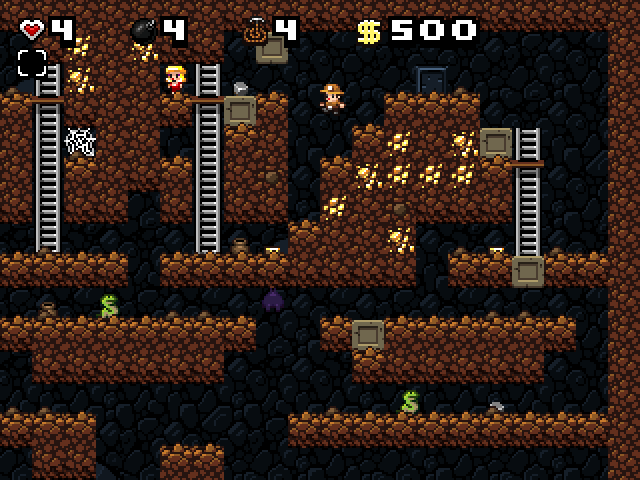
\includegraphics[width=.65\textwidth]{fig/spelunky-pc-screen.png}
\caption
    {\label{fig:spelunky-gameplay}Exemplo de partida de spelunky, mostrando
    elementos do jogo como o jogador, a caverna, os inimigos, os tesouros,
    entre outros.}
\end{figure}

\subsection{Competição SpelunkBots}
% O framework A competição

TBD

\section{Agentes Racionais}

Um agente pode ser visto como todo e qualquer tipo de entidade que seja capaz de
perceber o ambiente onde está situado, através de seus sensores, podendo
executar ações nesse ambiente conforme sua necessidade através de seus
atuadores.
\cite{Russell:1995:AIM:193191}

Para exemplificar, podemos tomar como exemplo o ser humano, que consegue
perceber o ambiente através de seus olhos e ouvidos, por exemplo, conseguindo
agir no ambiente com suas partes do corpo, como braços, pernas, mãos e etc.
\cite{Russell:1995:AIM:193191}

Nesse contexto, um agente racional é um agente que toma as ações que o coloca
mais próximo de completar seus objetivos.

\subsection{Agentes Reflexivos}

Agentes reflexivos são agentes que executam ações baseados em alguma situação
percebida. Por exemplo, podemos ter um agente reflexivo que poderá fazer uma
postagem em uma rede social, dado que uma outra pessoa fez uma postagem. Tal
tipo de agente não ``pensará'' sobre a ação que está executando, simplesmente a
executará baseado no que percebeu anteriormente.

Estes agentes têm como principal característica não guardarem tipo algum de
informação das suas experiências passadas, sendo apenas reativos.

\subsection{Agentes com Memória}

Diferentemente dos agentes reflexivos, agentes com memória são capazes de
guardar informações sobre as experiências passadas, podendo fazer o uso das
mesmas para alcançar seus objetivos. A lembrança das experiência passadas
possibilita à um agente uma forma de aprender e melhorar, fazendo com que, por
exemplo, sejam evitadas ações não efetivas ou que seja escolhida, entre um
conjunto de possíveis ações, a que seja a mais efetiva para o agente.

\subsection{Agentes Baseados em Objetivos}

Além de ter memória, é necessário que um agente saiba quando o mesmo obteve
sucesso no que se propôs a fazer. Com isso, agentes baseados em objetivos
conseguem basear suas decisões - ações a tomar - com base na ação que o deixa
mais próximo de alcançar seus objetivos. O desafio desse tipo de agente é saber
como alcançar esse objetivo, podendo ser usadas técnicas de busca e planejamento
para determinar as possíveis ações a serem executadas para alcançá-lo.

\subsection{Agentes Baseados em Utilidades}

Para alguns tipos de agente, chegar no objetivo pode não ser suficiente,
podendo existir outros fatores na busca desse objetivo que possam influenciar no
resultado final do agente. Por exemplo, um agente que joga um determinado jogo
pode terminar o jogo com um determinado número de pontos, porém, é mais
satisfatório que o mesmo termine o jogo com o \textbf{maior} número de pontos
possível.

Portanto, tais tipos de agentes são capazes de medir os resultados de suas
ações, escolhendo as que, além de alcançar seu objetivo, façam o mesmo da melhor
maneira possível.

\subsection{Ambiente}

\begin{itemize}
    \item Falar o que é um ambiente, e como é a interação do agente com o mesmo
    \item Falar dos tipos de ambiente (determinístico, estocástico, etc.)
    \item Dar exemplos de ambientes
\end{itemize}

\subsection{Objetivo}

??? Talvez devamos explorar esse assunto junto de agentes ???
??? Ou simplesmente remover essa Seção, visto que esse conceito está ``implícito'' ???

\subsection{Estado}

??? Talvez devamos explorar esse assunto junto de agentes ???
??? Ou simplesmente remover essa Seção, visto que esse conceito está ``implícito'' ???

\subsection{Agentes BDI}

TBD

\section{Frameworks de Inteligência Artificial}

TBD

\subsection{Motivação}

TBD

\subsection{Exemplos de Frameworks e Competições}

TBD

\section{Planejamento}

TBD

\section{Aprendizado de Máquina}

TBD

\subsection{Q-Learning}

TBD

\subsection{SARSA}

TBD

\subsection{Deep Learning}

TBD
